%TODO Beispiele zu Ende sowie Vorlage BA überarbeiten, Main Datei überarbeiten, Bilder mit ChatGPT erstellen

\chapter{Einführung in LaTeX}
	\label{chap:einfuehrung}
	
	
\section{Schreiben des ersten Textes}
	\label{sec:erster_text}
Das hier wird die Musertlösung sein. Am liebsten erstelle ich Tabellen in LaTeX. Das mache ich in Abschnitt \ref{sec:tabellen}. Grafiken finde ich aber auch schön, daher binde ich die in Abschnitt \ref{sec:grafik} ein.
	
\section{Einbinden von Objekten/Paketen}
	\label{sec:objekte}

	
\subsection{Die erste Grafik einfügen}
	\label{sec:grafik}
\begin{figure}[H]
	\centering
	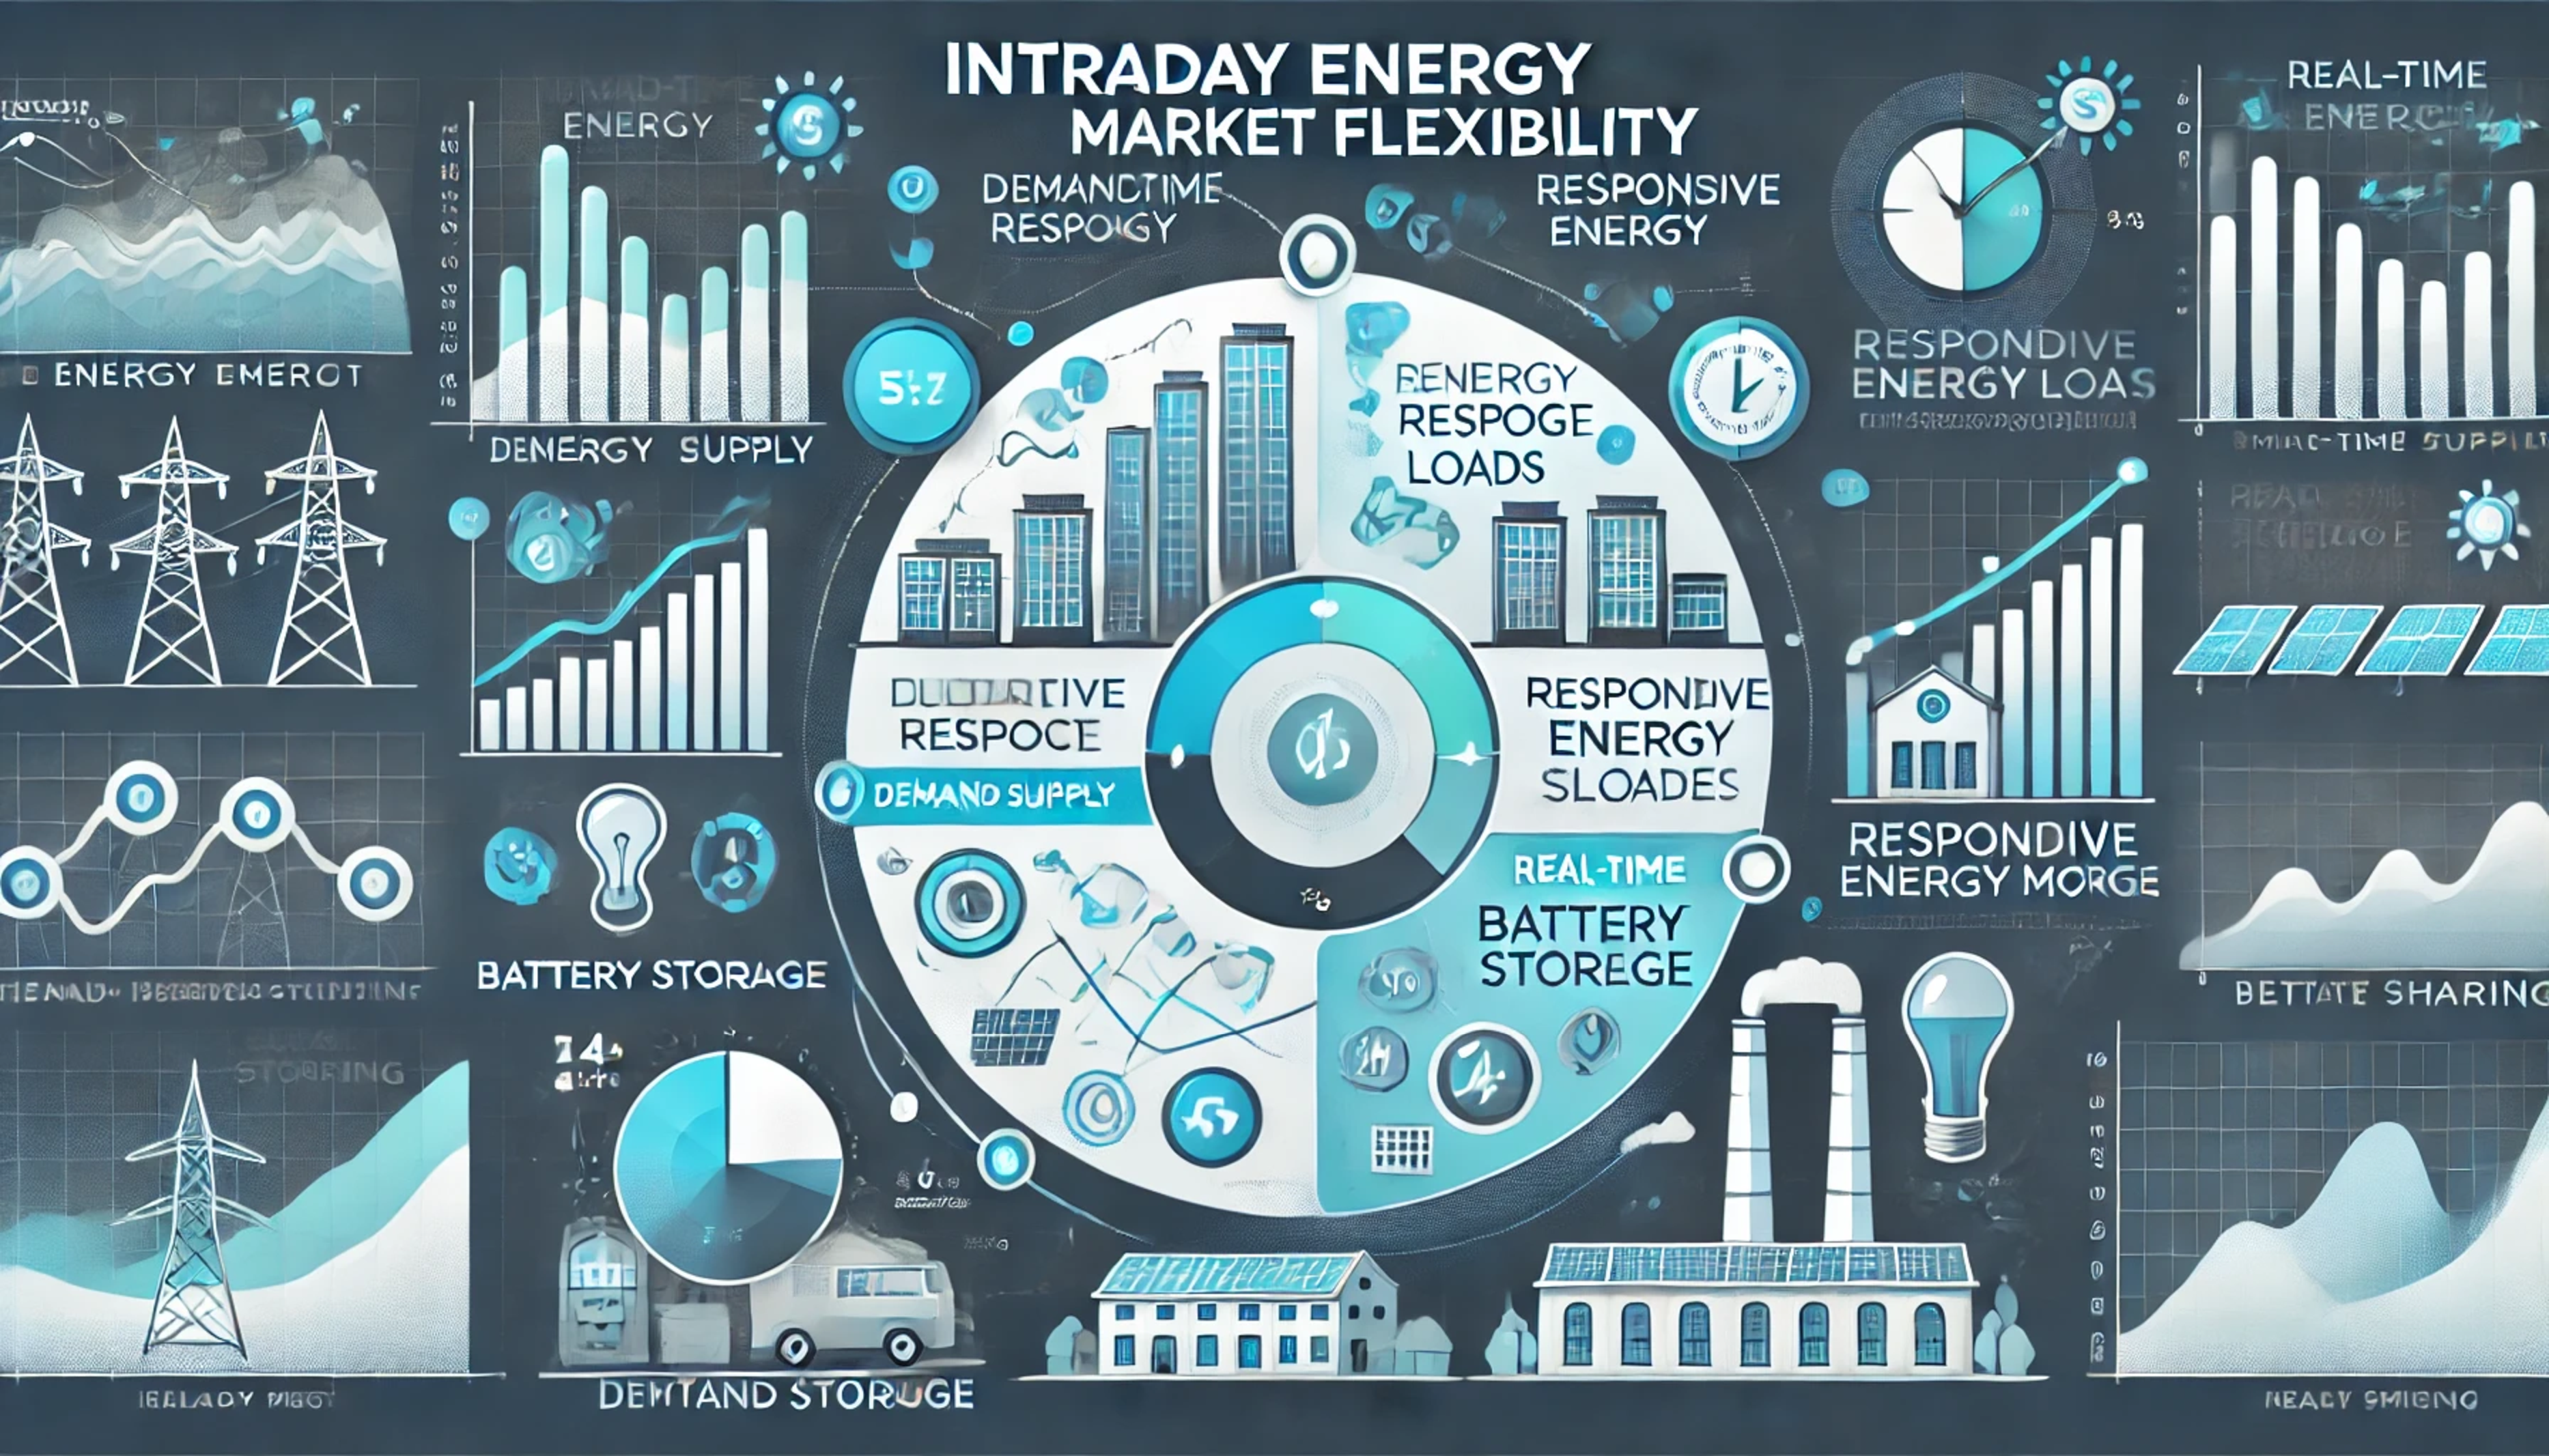
\includegraphics[width=0.9\linewidth]{bsp_pic.pdf}
	\caption[Titel fürs Inhaltsverzeichnis]{Titel unter Grafik mit Quelle 	\cite{openai2024chatgpt}}
	\label{fig:grafik_jpg}
\end{figure}

\begin{figure}[H]
	\centering
	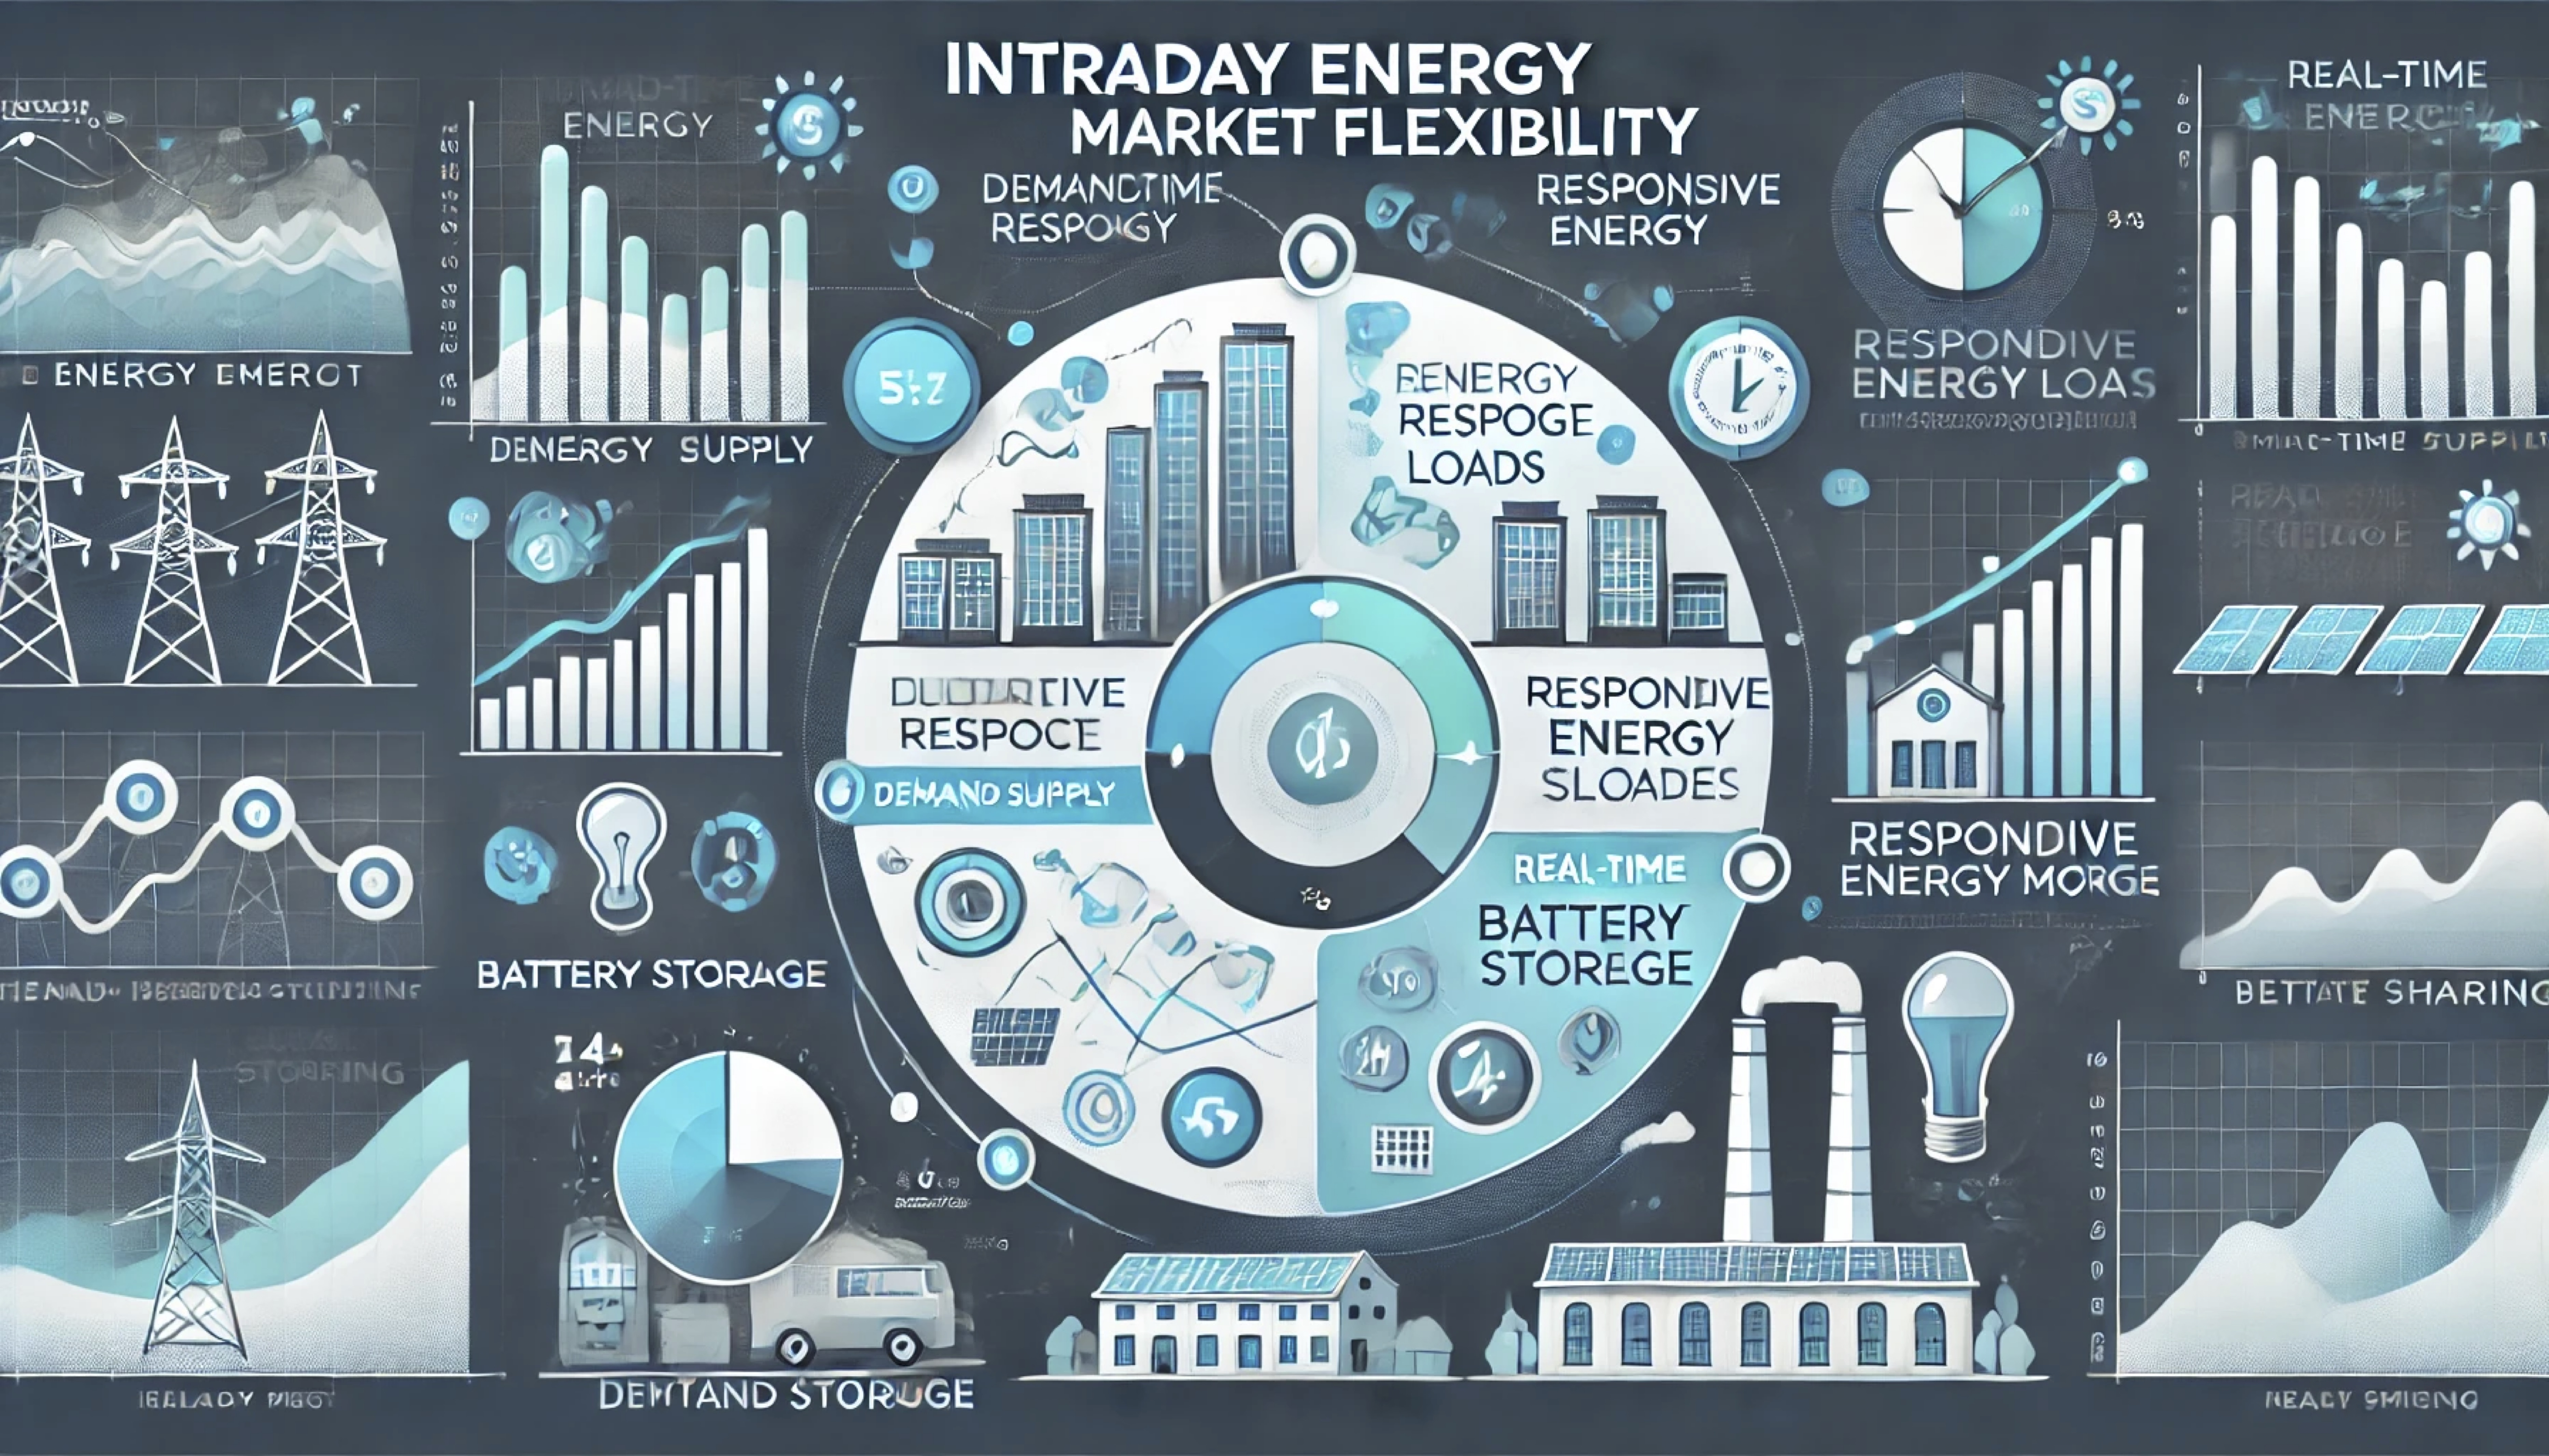
\includegraphics[width=0.9\linewidth]{bsp_pic.jpg}
	\caption[Titel fürs Inhaltsverzeichnis]{Titel unter Grafik mit Quelle \cite{openai2024chatgpt}}
	\label{fig:grafik_pdf}
\end{figure}
	
\subsection{Aufzählungen füge ich hier ein}
	\label{sec:aufzaehlung}

\begin{itemize}[noitemsep, label=+]
	\item Wärmepumpe
	\item Gaskessel 
	\item BHKW
	\item Gasturbine
\end{itemize}

\begin{enumerate}[noitemsep, label=\alph*]
	\item Wärmepumpe
	\item Gaskessel 
	\item BHKW
	\item Gasturbine
\end{enumerate}
	
\subsection{Tabellen können kompliziert sein}
	\label{sec:tabellen}
\begin{table}[H]
	\centering
	\caption{Dies ist die erste Tabelle}
	\label{tab:uebung1}
	\begin{tabular}{l|c|r}
		Bezeichnung&Werte&Einheit \\\hline
		Gaskraftwerk&10&MW\\
		Wärmepumpe&5&MW\\
	\end{tabular}
\end{table}	

\begin{table}[H]
	\newcolumntype{Z}{>{\centering \arraybackslash}X}
	\caption{Dies ist die zweite Tabelle}
	\label{tab:uebung2}
	\renewcommand{\arraystretch}{1}
	\scriptsize
	%	\rotatebox{90}{
		\begin{tabularx}{\textwidth}{|Z|Z|c|c|c|}
			\hline
			&&\textbf{Ausgangsszenario}&\multicolumn{2}{c|}{\textbf{Szenario 1.1}}\\\hline
			&Zinssatz & Invest.\,100\,\% &Invest.\,100\,\%&  Invest.\,60\,\%\\
			\hline
			\hline
			\multirow{3}{*}{\shortstack[c]{ \textbf{LCoH }\\ \textbf{15 Jahre}\\in \euro/MWh}} & 3\,\% & 80	&90&100
			\\
			\cline{2-5}
			& 5\,\% & 90		&	100	&	110
			\\
			\cline{2-5}
			& 8\,\% & 100		&	110	&	120
			\\
			\hline		\end{tabularx}
		%}
\end{table}

	
\subsection{Formeln kann ich auch gebrauchen}
	\label{sec:formeln}
\begin{equation}
	\label{eq:sum}
	min \sum_{t}^{8760} (K^{var. Gaskessel}_{t} + K^{var.W{"a}rmepumpe}_{t})
\end{equation}
	
\begin{align}
	&\dot{Q}^{Speicher,min} \leq \dot{Q}^{laden}_{t} \leq \dot{Q}^{Speicher,max}&\forall t \in T \label{eq:opt_grenze_beladen_speicher}\\
	&\dot{Q}^{Speicher,min} \leq \dot{Q}^{entladen}_{t} \leq \dot{Q}^{Speicher,max} &\forall t \in T \label{eq:opt_grenze_entladen_speicher}\\
	&Q^{Speicher}_{t=0} = Q^{init, sp} \cdot Q^{Kapzit \ddot{a} t}& \label{eq:opt_start_speicher}\\
	&Q^{Speicher}_{t=8760} \geq Q^{init, sp} \cdot Q^{Kapzit \ddot{a} t} & \label{eq:opt_end_speicher}
\end{align}


\section{Hier lerne ich zitieren}
	\label{sec:zitieren}
	
So kann ich etwas zitieren \cite{openai2024chatgpt}. Das wichtige ist, dass ich weiß wie ich citavi einbinde.
	
	
\chapter{Tipps und Tricks}
	\label{chap:tipps}
	
Hier binde ich einen Link ein ...\href{https://forschung.hs-kempten.de/de/forschungsprojekt/482-heatshift}{\enquote{ HeatSHIFT}}.\\
CO\textsubscript{2}-Kosten. \\
\textbf{Das wird Fett}

\textit{Das ist kursiv}

\enquote{Text}

$\left( Grosse Klammern\right)$

Groß\-wärme\-pumpen

\euro

\pagebreak

~ (Tilde)
Wert und Einheit werden nicht getrennt 200~kW
%

\mbox{Ich will das nicht trennen}

\href{link}{Text}

\footnote{Text}
Erstell Fußnote

